%% Exemple de source LaTeX pour un article soumis à TALN
\documentclass[10pt,a4paper,twoside]{article}

\usepackage{times}
\usepackage[utf8]{inputenc}
\usepackage[T1]{fontenc}
\usepackage{graphicx}

\usepackage{hyperref}
\usepackage{alltt}
\usepackage{amsmath}


% faire les \usepackage dont vous avez besoin AVANT le \usepackage{taln2014} 

% % % % % % % % % % % % % % % % % % % % % % % % % % % % % % % % % % % % % % % %
% 
\usepackage{taln2014}
\usepackage[frenchb]{babel}
%
% % % % % % % % % % % % % % % % % % % % % % % % % % % % % % % % % % % % % % % %


% Titre complet
\title{Désambiguïsation des relations de traductions dans DBNary}

\author{Untel Trucmuche\up{1, 2}\quad Unetelle Machinchose\up{1, 3}\\
  (1) LPL, AMU, CNRS, 5 avenue Pasteur, 13100 Aix-en-Provence \\ 
  (2) LIF, AMU, CNRS, 163 avenue de Luminy, 13288 Marseille Cedex 9\\ 
  (3) Lab, adresse, CP Ville, Pays \\ 
  utrucmuche@lpl-aix.fr, umachinchose@adresse-academique.fr \\ 
}

% Titre qui apparait en en-tête (1 ligne maxi)
\fancyhead[CO]{Modèle de document pour TALN 2014} 
% Auteurs qui apparaissent en en-tête (1 ligne maxi)
\fancyhead[CE]{Untel Trucmuche, Unetelle Machinchose} 

\DeclareMathOperator*{\argmax}{arg\!\max}

% % % % % % % % % % % % % % % % % % % % % % % % % % % % % % % % % % % % % % % %

\begin{document}

\maketitle


\resume{
Le projet DBNary a pour but de fournir des données lexicales liées extraites de différentes éditions de Wiktionary. À l’heure actuelle, 10 langues sont extraites, avec plus de 3.16 millions de liens de traduction qui connectent les entrées lexicales de ces langues vers des entrées dans plus de 1000 langues. Dans Wiktionary des gloses sont souvent associées aux traductions, ce qui aide l’utilisateur à comprendre à quel sens elles correspondent. Nous avons pour but d’extraire cette information et de désambiguïser les liens de traduction. Nous adaptons des mesures de similarité textuelle et sémantiques basée sur des intersections de gloses floues à cette fin. Nous extrayons enfin des numéros de sens, présents dans un sous ensemble des gloses, pour construire une référence d’évaluation endogène. Nous obtenons des F-mesures à la hauteur de travaux similaire (sur l’anglais) pour les trois langues testées (Français, Portugais, Finnois).
}
\\

\abstract{
The DBnary project aims at providing Lexical Linked Data extracted from Wiktionary editions. Data from 10 languages is currently extracted with over $3.16$M translation links that connect lexical entries to entries in more than a thousand languages. 
In Wiktionary, glosses are often associated with translations to help users understand to what sense they correspond. We aim to extract of as much of this information as possible and then to disambiguate the translations for available languages. We adapt textual and semantic similarity techniques based on fuzzy gloss overlaps to disambiguate the translation relations. We extract some of the sense number information present in glosses to build a gold standard for tuning and evaluation.
 We obtain F-measures up to par with similar works (on English only), across the three languages where we generated a gold standard (French, Portuguese, Finnish).
}
\\

\motsClefs{Wiktionary, Données léxicales liées, Ressource Multilingues}
{Wiktionary, Linked Open Data, Multilingual Resources}


%%================================================================
\section{Introduction}

 Wiktionary est une ressource lexico-sémantique construite collaborativement sous l'égide de la Fondation Wikimedia (qui héberge également la célèbre initiative Wikipedia). C'est actuellement la ressource collaborative de données lexicales la plus grande. Les pages Wiktionary décrivent habituellement des entrées lexicales en donnant leurs catégories grammaticales, un ensemble de définitions, des exemples, des relation lexico-sémantiques ainsi que des traductions dans plus de mille langues.

Le projet DBNary \cite{serasset:dbnary-swj} a pour objectif de fournir des données lexicales liées de haute qualité extraites des éditions en différentes langues de Wiktionary. DBNary permet actuellement d'extraire des données issues de 10 éditions et regroupe $3,16$ millions de liens de traduction qui mettent en relation les entrées lexicales des 10 langues extraites vers des entrées dans plus de mille langues. Ces chiffres sont en augmentation constante, sachant que le jeu de données DBNary est extrait dès que Wikimedia met à disposition de nouvelles archives des données (environs tous les 10 à 15 jours pour chaque langue).

La source de ces liens de traduction sont des \emph{entrées lexicales}. Le but de ce travail est d'attacher ces traductions au sens de mot correct correspondant et d'ainsi augmenter la valeur et la qualité de DBNary.
Des travaux similaires ont été menés (principalement dans le jeu de données Uby), mais sont limités à l'anglais et l'allemand. Dans cet article, nous avons travaillé avec les éditions de 9 langues, pour lesquelles nous avons du faire face aux habitudes hétérogènes des différentes communautés Wiktionary qui s'exprimaient par différentes propriétés linguistiques mises en avant. 

Après une présentation de la structure de DBNary, nous passons en revue les travaux similaires, suite à quoi nous expliquons comment nous construisons une référence endogène utilisée pour évaluer notre travail, nous détaillons les méthodes employées pour atteindre notre but, pour finir sur l'évaluation de notre méthode et de l'interprétons les résultats.

\section{Le jeu de données DBNary}

DBnary est un jeu de données liées ouvertes extraites depuis 10 éditions de langues Wiktionary (Anglais, Finnois, Français, Allemand, Grec, Italien, Japonais, Portugais, Russe, Turque). La ressource est disponible en ligne à l'adresse \url{http://kaiko.getalp.org/about-DBnary}. Au moment de l'écriture, DBnary contiens  plus de  35 millions de triples. Ce nombre à constamment augmenté au long de l'évolution du jeu de données au rythme des évolutions des données originales de Wiktionary. En effet, DBnary est automatiquement mis-à-jour dès que Wikimedia met à disposition une nouvelle version des archives Wiktionary, c'est-à-dire à peu près tous les 10 à 15 jours.

DBNary est structuré en suivant le modèle de l'Ontologie LEMON pour la représentation de données lexicales liées \cite{DBLP:conf/esws/McCraeSC11}. Le tableau \ref{lemon-elts} donne une idée du nombre d'éléments lexicaux tels que définis dans l'ontologie LEMON dans les différents éditions de langues.

Les éléments dans DBnary qui n'ont pu être représentés en LEMON, on été définis dans une ontologie sur mesure construite sur la base des classes et relations LEMON, notablement les relations lexico-sémantiques ainsi que ce que nous appelons des \verb|Vocables|, les entrées de haut-niveau dans Wiktionary qui correspondent aux pages Wiktionary pour des mots spécifiques et qui contiennent plusieurs entrées lexicales (\verb|LexicalEntry|) catégorisées en deux niveaux:
\begin{enumerate}
	\item Distinction de mots homonymes selon l'origine étymologique (par exemple: \verb|mode [la mode actuelle]|) contre \verb|mode [le mode de fonctionnement]|.
	\item Pour chaque origine étymologique différente, distinction selon la catégorie grammaticale (par exemple \\ \verb|rouge#Adj [la voiture rouge]| contre \verb|rouge#Nom [le rouge au front]|)
\end{enumerate}

\begin{table*}[htb!]
\begin{center}\begin{footnotesize}
\begin{tabular}{lrrrrrrr}
\textbf{Langue} & \textbf{Entrées} & \textbf{LexicalSense} & \textbf{Traductions} & \textbf{Gloses} & \textbf{Texte} &  \textbf{Nbr. de sens} & \textbf{Texte + Nbr. de sens }\\
\hline
Anglais & $544,338$ & $438,669$ & $1,317,545$ & $1,288,667$ & $1,288,667$ & $515$ & $515$ \\
Finnois & $49,620$ & $58,172$ & $121,278$ & $120,728$ & $120,329$ & $115,949$ & $115,550$ \\
Français & $291,365$ & $379,224$ & $504,061$ & $136,319$ & $135,612$ & $28,821$ & $28,114$ \\
Allemand & $205,977$ & $100,433$ & $388,630$ & $388,553$ & $3,101$ & $385,452$ & $0$ \\
Grec Moderne & $242,349$ & $108,283$ & $56,638$ & $8,368$ & $8,368$ & $12$ & $12$ \\
Italien & $33,705$ & $47,102$ & $62,546$ & $0$ & $0$ & $0$ & $0$ \\
Japonais & $24,804$ & $28,763$ & $85,606$ & $22,322$ & $20,686$ & $4,148$ & $2,512$ \\
Portugais & $45,109$ & $81,023$ & $267,048$ & $74,901$ & $72,339$ & $71,734$ & $69,172$ \\
Russe & $129,555$ & $106,374$ & $360,016$ & $151,100$ & $150,985$ & $115$ & $0$ \\
Turque & $64,678$ & $91,071$ & $66,290$ & $53,348$ & $585$ & $52,901$ & $138$ \\

\hline
\end{tabular}
\caption{Nombre d'éléments dans le jeu de données DBnary actuel avec des détails sur le nombre d'entrées et de sens de mot ainsi que le nombre de traduction. Le tableau détaille également le nombre de gloses rattachées à des traduction, et de manière plus précise le nombre de gloses textuelles, le nombre de gloses qui contiennent un numéro de sens et enfin le nombre de gloses qui contiennent à la fois une description textuelle et un numéro de sens.}
\label{lemon-elts}
\end{footnotesize}\end{center}
\end{table*}

\subsection{Relations de traduction}

DBnary utilise une représentation \textit{ad-hoc} pour les relations de traduction, sachant que le modèle LEMON ne propose pas de vocabulaire pour représenter une telle information.  \verb|Translation| est une ressource RDF qui rassemble toute l'information se rapportant aux relations de traduction. Par exemple, l'une des traductions de l'entrée lexicale de \emph{frog} est représentée comme suit : \footnote{Dans cet article ainsi que pour les jeux de données DBNary la syntaxe RDF Turtle est utilisée.}:

\begin{small}
\begin{alltt}
eng:__tr_fra_1_frog__Noun__1
      a       dbnary:Translation ;
      dbnary:gloss "amphibian"@en ;
      dbnary:isTranslationOf
              eng:frog__Noun__1 ;
      dbnary:targetLanguage
              lexvo:fra ;
      dbnary:usage "f" ;
      dbnary:writtenForm "grenouille"@fr .
\end{alltt}
\end{small}

Les propriétés de cette ressource pointent vers une source de type \verb|LexicalEntry|, la langue de la cible (représentée comme une entrée \verb|lexvo.org| \cite{deMeloWeikum2008c}), la forme de surface de la cible, et 'éventuellement une glose et des notes d'usage. 
Les notes d'usage donnent des informations sur la cible de la traduction (habituellement le genre où la transcription de la cible).

La glose donne une information de désambiguïsation sur la source de la traduction. Dans l'exemple donné, il est dit que la traduction ne correspond qu'au sens de \emph{frog} qui peut être décrit par l'indice ``\emph{amphibian}''. Certaines de ces gloses sont textuelles et résument ou reprennent la définition ou une partie de celle-ci d'une ou plusieurs sens de la source auxquels s'applique la traduction.

Par exemple , la \verb|LexicalEntry| Anglaise \emph{frog} contient huit sens de mots définis comme suit : 

\begin{small}\begin{enumerate}
\item A small tailless amphibian of the order Anura that typically hops
\item The part of a violin bow (or that of other similar string instruments such as the viola, cello and contrabass) located at the end held by the player, to which the horsehair is attached
\item (Cockney rhyming slang) Road. Shorter, more common form of frog and toad
\item The depression in the upper face of a pressed or handmade clay brick
\item An organ on the bottom of a horse’s hoof that assists in the circulation of blood
\item The part of a railway switch or turnout where the running-rails cross (from the resemblance to the frog in a horse’s hoof)
\item An oblong cloak button, covered with netted thread, and fastening into a loop instead of a button hole.
\item The loop of the scabbard of a bayonet or sword. 
\end{enumerate}\end{small}

Les traductions de cette entrée sont divisées en quatre groupes correspondant aux gloses ``\emph{amphibian}'', ``\emph{end of a string instrument’s bow}'', ``\emph{organ in a horse’s foot}'' et ``\emph{part of a railway}''.

De plus, parmi les gloses, certaines peuvent contenir des numéros de sens, ajoutés par des utilisateurs de manière ad-hoc (peuvent ou non être présentes, et même si elles le sont, aucun format systématique n'est suivi ou imposé.) Il en suit que la présence d'information de désambiguïsation est très irrégulière et très variable entre les différentes éditions de langues, à la fois en termes de la structure du wiki et de la représentation. 


Dans l'état courant de l'extracteur Wiktionary, nous extrayons toutes les traductions, et quand c'est possible les gloses associées.  Néanmoins, jusqu'à présent nous n'avions pas exploités l'information contenue dans les gloses pour enrichir et désambiguïser les sens source des relations de traduction.


Comme nous l'avons déjà mentionnés, le contenu et le format des gloses est très variable selong les langues, tant qualitativement qie quantitativement.

En effet, comme le montre le tableau \ref{lemon-elts}, certaines langues telles que l'italien ne contiennent aucunement de gloses, pour d'autres, comme l'anglais, il y a des gloses textuelles mais pas de numéros de sens. Pour d'autres encore, telles que l'allemand ne contiennent presque pas de gloses textuelles, mais donnent systématiquement le numéro de sens. Dans les cas spécifique du français, du finnois et du portugais, beaucoup de liens de traductions ont à la fois une glose textuelle rattachée et une numéro de sens.

Dans le but d'évaluer notre méthode, nous avons décidé d'exploiter ces gloses qui contiennent à l fois une description textuelle et un numéro de sens.


\subsection{Création d'une référence d'évaluation}
Il arrive souvent que parmi les gloses de traduction disponibles qui contiennent une information textuelle ou un numéro de sens qu'il y ait des faux positifs à la fois du à une extraction approximative à cause de la variabilité des la structure des gloses. Avant d'aller plus loin il est essentiel de filtrer l'information présente afin de ne conserver que les parties pertinentes.

Plus concrètement, deux étapes sont nécessaire pour mener à bien l'extraction des informations nécessaires:
\begin{itemize}
	\item Supprimer les gloses vides ou contenant des informations textuelles non pertinentes qui correspondent souvent à des notes de type \emph{à faire} (par ex. ``\emph{traduction à vérifier}'').
	\item Extraire les numéros de sens des gloses qui en possèdent un, en utilisant des patrons spécifiques à chaque langue (par ex. ``\emph{glose textuelle (1)}'' ou ``\emph{1. glose textuelle}'')
\end{itemize}


Une fois il y avait quantité suffisante de ces gloses (dans telle ou telle édition de langue) nous avons supprimés les numéro s de sens\footnote{Les traductions correspondent parfois à plusieurs sens} des gloses, et les avons utilisées pour produire un étalon-or suivant le format du programme d'évaluation de trec\_eval.

Après cet étape d'extraction, ont peut désormais passer à la description du processus de désambiguïsation à proprement parler. Même si l'extraction était spécifique à chaque langue, la méthode de désambiguïsation a été conçue pour être aussi générique et calculatoirememnt efficiente que possible, sachant que l'on est amenés à effectuer la désambiguïsation périodiquement dès qu'une nouvelle version de DBnary est extraite de Wiktionary.



\section{Travaux Similaires}

\subsection{Extraction de données depuis les éditions de Wiktionary} Depuis sa création en 2002, Wiktionary à connu une augmentation régulière en taille (à la fois par un travail collaboratif ainsi que l'insertion automatique de données lexicales libres précédemment disponibles). L'engouement pour Wiktionary en tant que source pour la production de données lexicales pour des applications du TAL s'est développé rapidement, et des études comme, par exemple \cite{Zesch:AAAI2008} où \cite{navarro-EtAl:2009:PeoplesWeb} démontrent la richesse et la puissance de ces ressources.

Depuis, les travaux se sont surtout concentrés sur l'extraction systématique de données provenant de Wiktionary.  La plus part de ces efforts d'extraction se font dans le cadre d'un  besoin pour ressource spécifique à un projet donné, et qui ne constituent ainsi qu'une capture de Wiktionary à un instant donné. Toutes les éditions de Wiktionary évoluent régulièrement (et indépendamment les unes des autres), y compris vis-à-vis de la manière dont sont représentées les données, de tels travaux ne peuvent pas fournir un accès durable aux données de Wiktionary.


Certains des travaux cependant demeurent maintenus, ce qui permet un accès au cours du temps. L'un de plus mature de ces travaux est l'API \emph{JWKTL} \cite{ZeschMuellerGurevych2008} qui donne accès aux éditions Anglaises, Allemandes et Russes. C'est cette dernière qui est utilisée dans le projet UBY \cite{gurevych2012uby}, qui met à disposition une version LMF de ces éditions.

Il faut également faire mention du projet wikokit \cite{krizhanovsky2010transformation}, qui donne accès  aux éditions Anglaises et Allemandes, et qui à été utilisée par \emph{JWKTL}.

\cite{HellmannSebastianandBrekleJonasandAuer} présentent un autre exemple, sous l'égide du projet dbpedia  \cite{dbpedia-swj}, dont l'objectif est en particulier de fournir un accès aux données de Wiktionary en tant que données liées ouvertes. La raison principale que rend cette approche intéressante, est l'aspect collaboratif, utilisé pour créer les patrons d'extraction, ce qui correspond à l'approche générale du projet dbpedia. Ce projet donne accès aux éditions de Wiktionary Anglais, Française, Russe et Allemande.

Cet article et les travaux effectués ici le sont dans le cadre du projet DBnary \cite{serasset:dbnary-swj}, dont l'objectif est similaire à celui de \cite{HellmannSebastianandBrekleJonasandAuer}. Plus précisément, notre objectif est de fournir une base de données lexicale au format LEMON, qui structure les données comme dans des lexiques traditionnels. En effet, nous extrayons des données issues de Wiktionary, en nous restreignant toutefois aux données ''natives'' de chaque édition. Par exemple, sont extraites les données en Français de l'édition Française, mais ignorons les données en Français contenues dans d'autres éditions.
À notre connaissance, DBNary est actuellement l'extracteur pour Wiktionary le plus avancé, avec son support actif courant de 10 langues. C'est également le seul projet qui donne accès à tout l'historique des données extraites. 

\subsection{Désambiguïsation des sources des liens de traduction} 

En ce qui concerne le rattachement des liens de traduction aux sens de mots les plus adéquats (déambiguïsation des liens de traduction), les travaux les plus similaires sont ceux de \cite{meyer-gurevych:2012:PAPERS}, dont les objectifs correspondent aux nôtres. Cependant leurs travaux portent seulement sur les éditions Anglaises et Allemandes. De plus, la référence utilisée pour évaluer leur méthode fut créé manuellement et est d'une taille significativement plus petite que notre référence endogène que nous avons ici extraite de la ressource elle-même.  Leur travail utilise également une stratégie de repli (vers le sens le plus fréquent), quand leurs heuristiques à base de mesures de similarité et sur la structure de la ressource échouent.  Leurs autres heuristiquet, impliquent également une analyse plus fine des définissions et gloses afin de notamment faire une distinction entre les étiquettes  linguistiques (domaine, registre, titre, etc.).

Dans le travail présenté, nous obtenons des résultats similaires sur les langues où nous avons la possibilité d'évaluer la désambiguïsation avec une référence endogène, même en utilisant seulement des mesures de similarité de chaines et de mots, et ce y compris dans les langues avec des propriétés moins communes (par exemple la nature agglutinante du Finnois.)  

\subsection{Mesures de similarité}
Notre méthode est basée sur l'application de mesures d'intersection de gloses et de leurs extensions avec des idées provenant des mesures de similarité textuelles hybrides, qui calculent une correspondance de sous-séquences à la fois au niveau du caractère et du mot. Dans les travaux cités ci-dessus, \cite{meyer-gurevych:2012:PAPERS}, une mesure de similarité à base de traits est utilisée (intersection de gloses), alors que dans leurs travaux antérieurs \cite{MeyerGurevych:2010}, ils ont utilisé une mesure de similarité textuelle basée sur des espaces vectoriels générés à partir de corpus (Analyse Sémantique Explicite).

Dans notre travail, nous proposons l'utilisation d'une mesure de similarité simple, où nous remplaçons la correspondance de mots exacte du calcul d'intersection par une mesure de distance de chaine approchée, et en nous plaçant dans le contexte plus général de la mesure de similarité qu'est l'indice de Tversky (qui peut être vu comme une généralisation de Lesk, du coefficient de Dice, des indices de Jaccard et Tatimono, etc.)

 L'idée de \emph{cardinalité molle} (``soft-cardinality'') proposée par \cite{Jimenez2010,Jimenez2012} est très similaire, dans le sens où elle exploite l'index de Tversky comme base et la conjugue avec une mesure de similarité textuelle. C'est à dire, au lieu d'incrémenter la cardinalité de l'intersection de 0 ou 1, elle est incrémentée par la valeur retournée par une mesure de similarité de chaine pour chaque paire de mots /?considérée lors du calcul de la cardinalité de l'intersection. 
 
  Leur mesure est basée sur la notion de q-grammes, générés empiriquement (caractère-grammes correspondant à des sous-chaines) avec une pondération à base de contenue d'information mutuelle ponctuelle (pointwise mutual information). Dans note cas, construire ce type de modèle pour 10 langues nécessiterait de nombreux efforts, et avec l'extension future à plus de langues (voire toutes), cela deviendrait une tâche pratiquement impossible. 
 
 De ce fait, nous avons choisis une mesure de distance de chaine simple pour le calcul de la correspondance partielle de chaines. Cependant, il y a de nombreuses mesures disponibles et il advient de choisir celle qui est la plus appropriée pour notre tâche (voir Section \ref{sec:expe}). Qui plus est, il existe également des mesures dites de ``Niveau 2'' qui combinent déjà de différentes manières des mesures de similarité de chaines avec des mesure d'intersection de termes. Ainsi il faudra évaluer la méthode que nous proposons, avec certaines de ces mesures de ``Niveau 2'' existantes afin d'estimer le viabilité. Toutes ces mesures ont fait l' objet d'une évaluation et d'une comparaison extensive entre elles dans le contexte d'une tâche de correspondance de noms \cite{Cohen2003}.




\section{Lier les traductions aux sens}
\subsection{Formalisation du processus de désambiguïsation}
Soit \(T\) l'ensemble des relations de traduction, \(L\) l'ensemble des \verb|LexicalEntry| dans une édition de langue donnée de DBnary. Soit \(T_i\in T: Gloss(T_i)\) une fonction qui renvoie la glose d'une relation de traduction quelconque \(T_i\in T\) et soit \(Source(T_i)=L_{T_i}\) une fonction qui renvoie une référence vers la \verb|LexicalEntry| source \(L_{T_i}\) d'une relation de traduction quelconque \(T_i\). soit \(Senses(L_i)=S_{L_i}\) l'ensemble des sens associées à une  \verb|LexicalEntry| \(L_i\). Soit \(S_{L_i}^k\) le \(k\)-ème sens contenus dans \(S_{L_i}\) et soit \(Def(S_{L_i}^k)\) une fonction qui renvoie la définitions textuelle d'un sens  \(S_{L_i}^k\). Enfin, soit \(Sim(A,B)\) une fonction qui renvoie  une mesure de similarité ou un score de relation sémantique  entre \(A\) et \(B\), où \(A,B\) est une paire de définitions textuelles ou de gloses textuelles. 

Ainsi, nous pouvons exprimer le processus de désambiguïsation comme:
\[
\forall T_i \in T, S=Senses(Source(T_i)): 
\]
\[
Source^*(T_i) \leftarrow  \argmax_{S^k\in S} \{Score(Gloss(T_i),Def(S^k))\}
\]

Ceci correspond exactement à une maximisation de la mesure de similarité \emph{a postériori} et résulte sur un sens désambiguïsé par lien de traduction. Cependant, il arrive dans de nombreux cas qu'un lien de traduction ne correspond à deux sens ou plus à la fois. La solution adoptée par \cite{MeyerGurevych:oup2012} est d'utiliser une valeur seuil \(k\) pour le calcul de la maximisation de la cardinalité de l'intersection des gloses. Dans notre cas, comme nous voulons évaluer et tester plusieurs mesures, sans que l'on puisse nécessairement garantir la normalisation des valeurs de sortie, un seuil \(k\) correspondant à une valeur fixe n'est pas garanti d'être approprié, même si dans la majorité des cas il faut se tenir à la contrainte que les valeurs des mesures de similarités soient normalisées entre  \(0 \mbox{ et  } 1\).

Au lieu de prendre un \(k\) fixe nous avons choisi d'utiliser une fenêtre \(\delta\) autour du sens sélectionné avec le score maximum, ce qui est plus robuste, notamment dans les cas où les valeurs de similarités ne sont pas sur la même échelle. Tout autre sens tombant dans la fenêtre est aussi accepté comme désambiguïsation.  

En comparaison, l'effet d'utiliser une valeur seuil fixe est que si tous les scores sont bas, aucun sens ne sera assigné, on gagne ainsi en précision au prix d'un rappel inférieur. C'est un comportement qui est en temps normal désirable, car détecter les erreur a postériori est difficile, cependant dans le cadre de cette expérience, garder les choix erronés en cas de scores bas nous permet ensuite à l'aide de la référence de repérer précisément les erreurs potentielles et de mieux les analyser et identifier leur origine exacte. 

Pour intégrer le seuil, nous pouvons modifier la fonction \(argmax\) comme suit:
\[
\forall T_i \in T, S=Senses(Source(T_i)): 
\]
\[
M_S = \max_{S_k\in S}(Score((Gloss(T_i),Def(S^k))),
\]
\[
\argmax_{S_i\in S}^\delta \{Score(Gloss(T_i),Def(S^k))\}=
\]
\[
\{S^k\in S|  M_S > Score((Gloss(T_i),Def(S^k)) > M_S-\delta \}
\]

\subsection{Mesure de similarité}
Afin de désambiguïser les relations de traduction, nous avons besoin de d'utiliser une mesure de similarité sémantique. Sachant que d'une part les seules informations disponibles sont les gloses qui représentent ou résument la définition du sens correspondant et sachant que d'autre part nous avons des définitions textuelles au niveau des sens, il nous faut une mesure de similarité qui ne se basent que sur les chaines de caractères et les mots. 
La mesure de Lesk \cite{citeulike:625530} est un mesure de similarité très simple et standard, qui s'adapte tout particulièrement aux contraintes auxquelles nous sommes confrontés. Cette mesure calcule dans sa formulation classique la cardinalité de l'intersection de deux ensemble de mots (typiquement des définitions de sens de mot).
 Cependant, vienne s'ajouter à cela un certain nombres de limitations importantes :
\begin{itemize}
	\item Si les tailles de gloses ou définitions n'est pas la même, cette mesure favorisera toujours les définitions plus longues. 
	\item La taille et l'adéquation des mots contenus dans les définitions est important, en effet, si il manque un mot clef dans la définition on peut facilement obtenir une similarité erronée (par exemple un score de zéro alors que l'idée est quand même la même, quand par exemple l'une des définition est formulée avec des synonymes du contenu de l'autre).  
	\item La mesure de Lesk classique c'est pas normalisée, c'est à dire que les valeurs peuvent être arbitrairement grandes. L'ajout d'une normalisation n'est pas toujours trivial, et dépend de nombreux facteurs, y compris le domaine d'application.
\end{itemize}
 
 
 Les problèmes de longueurs différentes de définitions et de la normalisation sont en réalité liés. Par exemple un moyen courant de normaliser la mesure est de diviser le score par la longueur de la définition la plus courte ou la plus longue.
 Un autre point intéressant est de remarquer la similarité entre la mesure de Lesk et les coefficients de Dice ou les indices de Jaccard/Tanimoto. En réalité toutes ces mesures sont des cas particulier du modèle plus général de l'indice de Tversky, qui provient des recherches sur la similarité en psychologie cognitive par A. Tversky \cite{tversky77similarity}.

L'indice de Tversky peut être défini de la manière suivante. Soit \(s_1 \in Senses(L_1)\)  et \(s_2 \in Senses(L_2)\), les sens de deux entrées lexicales \(L_1\) et \(L_2\). Soit \(d_i=Def(s_i)\) la définition de \(s_i\), représentée par un ensemble de mots. Alors, la similarité \(Score(s_1, s_2)\) entre les sens s'exprime comme :
\[
Score(s_1,s_2) = 
\frac{|d_1\cap d_2|}{|d_1\cap d_2| + \alpha |d_1-d_2| + \beta |d_2-d_1|}
\]

La mesure peut être généralisée d'avantage en suivant la proposition de \cite{DBLP:conf/otm/PirroE10} en remplaçant la fonction de cardinalité par une fonction quelconque \(F\). Selon les valeurs d'\(\alpha\) et de \(\beta\), l'indice de Tversky prends, comme nous l'avons mentionnés la forme d'autres indices ou coefficients. Pour \((\alpha=\beta=0.5)\) il est équivalent au coefficient de  Dice, et pour \((\alpha=\beta=1)\) à l'indice de Tanimoto. Plus généralement les valeurs de   \(\alpha\) et \(\beta\) expriment combien d'emphase ont attribue aux points communs ou aux différences d'un sens ou de l'autre.

L'indice de Tversky en lui même n'est pas une mesure où une similarité dans le sens mathématique du terme, car en effet il n'est n'y symétrique, ni ne respecte l'inégalité triangulaire, cependant une formulation symétrique à été proposée par 
\cite{Jimenez2010}  pour les cas où c'est une propriété qui est requise. 
% : 
% 
% \[
% S(s_1,s_2) = \frac{|d_1\cap d_2|}{|d_1\cap d_2| + \beta (\alpha a + (1-\alpha)b)}\]
% \[
% a=min(|d_1\cap d_2|,|d_2\cap d_1|)\\
% \]\[
% b=max(|d_1\cap d_2|,|d_2\cap d_1|)\\ 
% \]
 
 Lors de l'utilisation de l'index de Tversky où des ces variantes, une attention toute particulière doit être portée au choix des poids, car selon les applications différents poids vont avoir une très grande influence sur les résultats. 

Dans notre contexte, nous n'avons pas de besoin particulier que la mesure soit symétrique, nous nous cantonnons donc à la forme de base de l'indice. 
 
\subsubsection{Contexte Multilingue et cardinalité partielle}
Quand on travaille sur une seule langue tel que l'Anglais ou le Français, nous avons à notre disposition des outils tels que des lematiseurs, ou encore des racinisateurs, qui peuvent aider à normaliser les formes de mots présentes à une représentation canonique. Ainsi nous pouvons espérer maximiser les cardinalité d'intersection en réduisant la parcimonie habituelles des définitions de sens ou encore plus des gloses. 

De plus pour dans langues agglutinantes telles que le finnois ou l'allemand où encore pour des langues fléchies (par exemple dans la langue Bangalie, les racines communes ne font souvent qu'un caractère, ce qui rends la racination difficile à exploiter) ou encore les langue avec une segmentation non triviale, ces étapes de pré-traitement sont essentielles afin de rendre les mesures de similarité à base l'intersection viables. Dans le contexte de DBNary, nous travaillons avec 10 langues, et le outils mentionnés si-dessus ne sont pas disponibles pour toutes, et même si ils l'étaient, les rassembler pour toute les langues est une tâche ardue. De ce fait nous avons choisi de ne pas présupposer l'existence de ces outils, mais au contraire de considérer qu'ils n'existent pas et de trouver une méthode alternative.

En temps normal, lors du calcul du score Lesk, si deux mots des définitions correspondent on augmente le score de 1 et sinon le score ne change pas. Cependant, si on remplaçais la correspondance exacte des mots par une mesure de distance de chaine qui mesurerais alors une distance approximative entre les paires de mots des définitions, on pourrais alors obtenir une mesure de Lesk ``floue''. C'est une approche très simple qui a un grand potentiel d'un point de vue de sa performance, en effet la méthode similaire de \cite{Jimenez2012} mène déjà à des bons résultats dans le contexte de la similarité textuelle. Il reste à évaluer et quantifier le potentiel pour la désambiguïsation de relations dans un contexte multilingue.

Comme il a été mentionné dans la parties sur les travaux similaires, il existe de nombreuses mesures de distance approchées entre chaines, comme évalué et mis en avant par \cite{Cohen2003}.
Nous pouvons intégrer dans l'indice de Tversky ces mesures, en remplaçant la fonction \(F\)de manière adéquate. En somme il s'agit d'une version simplifiée de la formulation de \cite{Jimenez2012}, où \(sim\) est une mesure de chaine approchée:

\[
	A \mbox{ , a set} : F(A) = (\sum_{A_i,A_j \in A}sim(A_i, A_j))^{-1}
\]


\subsubsection{Contraintes liées à la plus longue sous séquence commune}
Avec cette mesure de similarité approchée, nous cherchons principalement à identifier les racines communes entre les mots sans utiliser de racinisateur. De ce fait, nous ne voulons par exemple pas considérer des préfixes ou suffixes, car ils ne portent pas l'information sémantique principale du mot en question. Si les mots des définitions n'ont en commun qu'un même suffixe qui revient souvent, nous aurons un score artificiellement haut, sans tout de même capturer dans d'information sémantique. Une première solution à ça, bien que partielle et de poser l'hypothèse de travail que les racines ont au moins trois caractères en commun dans une sous séquence contigüe et ainsi mettre le score à zéro si la plus longue sous séquence commune est de longueur inférieure à trois.

\section{Expériences}
\label{sec:expe}
Comme décrit précédemment, nous avons pu extraire des gloses avec des numéros de sens, une référence pour certaines éditions de langues Wiktionary, où les informations étaient présentes en quantité suffisante. Nous avons alors enlevés les numéros de sens des gloses afin de pouvoir faire tourner notre algorithme de désambiguïsation sur les traductions en question, et ensuite évaluer les résultats vis-à-vis de la référence.

Nous décrivons ici d'abord plus en détail comment nous avons généré la référence et les outils et mesures utilisés pour l'évaluation. 
Nous passerons ensuite à la description de notre méthodologie et des résultats pour l'estimation des paramètres optimaux pour notre indice de Tversky, ainsi que l'estimation de la mesure de chaine approchée optimale à utiliser pour le calcul de la cardinalité approchée. Enfin nous comparons cet index de Tversky optimal avec d'autre mesure de similarités dites de ``Niveau 2''
 
\subsection{Évaluation}
\subsection{Référence d'évaluation}
Seulement certaines éditions de langues réunissaient les conditions nécessaires pour la génération d'une référence de taille acceptable: 
\begin{enumerate}
	\item Des gloses textuelles sont présentes
	\item Les gloses en questions contiennent également un numéro de sens.
	\item Les éléments des deux points précédents sont présents en quantité suffisante (au moins quelques milliers)
\end{enumerate}

Quatre éditions de langues réunissent les conditions ci-dessus (voire l'ultime colonne de  la table \ref{lemon-elts}): français, portugais, finnois et japonais, cependant le japonais possédant bien moins de gloses adéquates, nous avons choisi de l'écarter afin que les résultats soient calculés sur des quantités de données du même ordre de grandeur.

\subsubsection{Trec\_eval, l'évaluation comme tache de questions-réponses}

une tâche de questions-réponses est plus précisément un problème d'étiquetage multiple, ce qui est exactement équivalent aux résultats que nous produisons avec le seuil \(\delta\). Nous pouvons considérer que chaque numéro de traduction est un identifiant de requête et que l'URI de chaque sens est un identifiant de document. Nous pouvons ainsi répondre aux requêtes  "traductions" en fournissant comme réponses une où plusieurs URI correspondant aux sens désambiguïsés ainsi que des poids associés. 

Si nous représentons maintenant l'étalon et les réponses dans le format de l'évaluateur Trec\_eval, nous pouvons ainsi utiliser ce dernier pour calculer tous les scores pour l'évaluation de notre désambiguïsation.

\subsubsection{Mesures d'évaluation}
Nous utiliserons les mesures standard de correspondance d'ensemble des domaines de la recherche d'information et de la désambiguïsation lexicale, c'est-à-dire la précision, le rappel et la F-mesure. Où \(P=\frac{|\{Pertinent\}\cap\{Désambiguïsé\}|}{|\{Désambiguïsé\}|}\), \(R=\frac{|\{Pertinent\}\cap\{Désambiguïsé\}|}{|\{Pertinent\}|}\), et \(F_1 = \frac{2\cdot P \cdot R}{P + R} \), la moyenne harmonique de \(R\) et \(P\). Cependant, pour la première étape d'estimation de paramètres nous n'utiliserons que la F-mesure, suite à quoi nous détaillerons les autre mesures pour les résultats finaux.
\subsection{Réglages de la mesure de similarité}

Il y a plusieurs paramètre à fixer avant de pouvoir utiliser l'indice de Tverski proposé, mais la première étape sera de déterminer quelle est la meilleure mesure approchée de distance de chaîne.

\subsubsection{Distance de chaine optimale}
 Le paramètre \(\delta\) influence la performance  indépendamment de la mesure de similarité, nous pouvons donc, dans un premier temps \(\delta=0\), ce qui met une restrictions  à une seule désambiguïsation par relation de traduction. De plus, les poids de l'indice de Tversky sont appliqués en aval de la mesure de distance de chaine approchée et n'influencent pas la performance relative due à telle ou telle mesure de chaine approchée. Ainsi, pour cette première expérience, nous fixons \(\alpha=\beta=0.5\), en d'autre mots, l'index de Tversky devient le coefficient de Dice.

Quant aux mesure de chaine approchées que nous considérons pour la comparaison, nous avons pris les mesures évaluées par  \cite{Cohen2003} qui avaient parmi les meilleures performances, en d'autre termes Jaro-Winkler, Monge-Elkan, Distance de Levenshtein mis à l'échelle. Nous considérons aussi la mesure de la sous-chaine commune la plus longue. Comme mesure de référence nous choisissons la mesure de Tverski avec une cardinalité d'intersection standard (correspondance complète).

Nous utilisons les notations suivantes pour les mesures: Tversky Index -- Ts; Jaro-Winkler -- JW; Monge-Elkan -- ME;  Levenshtein mis à l'échelle -- Ls; Sous-chaine commune la plus longue -- Lcss; F -- Flou/Approché. Par  exemple, la mesure de  Tversky standard avec une cardinalité classique porterait l'abréviation "Ti", alors que Tversky approché avec la mesure de distance de chaine de Monge-Elkan s'écrira "FTiME". 

La table \ref{tab:expe1} présente les résultats pour chaque mesure de chaine approché dans chacune des trois langues d'évaluation (Fr, Fi, Pt).

Comme nous pouvons le constater, la mesure de Levenshtein mise à l'échelle donne des valeurs de F-mesure systématiquement supérieurs de  \(+1\%\) à \(+1.96\%\) par rapport aux autres mesures de distance.

\begin{table}
{\centering \footnotesize
\begin{tabular}{|c|c|c|c|}
\hline &French&Portuguese&Finnish\\
\hline &F1&F1&F1\\
\hline FTiJW&0.7853&0.8079&0.9479\\
\hline FTiLcss&0.7778&0.7697&0.9495\\
\hline FTiLs&\textbf{0.7861}&\textbf{0.8176}&\textbf{0.9536}\\
\hline FTiME&0.7684&0.7683&0.9495\\
\hline Ti&0.7088&0.7171&0.8806\\
\hline 
\end{tabular} 
\caption{Scores  F\_1 score pour les différentes mesures de distance de chaine selon la langue (valeur maximale en gras).}
\label{tab:expe1}
}
\end{table}

\subsubsection{Sélection des \(\alpha\), \(\beta\) optimaux}

Maintenant que nous avons trouvé la distance de mesure de chaine optimale, nous pouvont chercher les valeurs optimales pour \(\alpha\) et \(\beta\). Ici, nous cardons les deux valeurs complémentaires, c'est-à-dire \(\alpha=1-\beta\) afin d'obtenir des scores équilibrés et entre zéro et un.

Sachant que les gloses des traductions sont courtes (souvent un mot unique), on peut faire l'hypothèse que l'optimal risque d'être aux alentours de \(\alpha=1-\beta=0.1\), car le plus important c'est que ce seul mot de la glose corresponde, la quantité des autres mots de la définitions importe peu.
Nous faisons varier les valeurs de  \(\alpha\) et \(\beta\) par pas de \(0.1\). La figure \ref{fig.1} montre de manière graphique  le score \(F\_1\) pour chaque pair de valeurs pour les trois langues. On vois bien que l'hypothèse était bien fondée et qu'avec \(\alpha=1-\beta=0.1\) il y a une différence entre \(+0.15\%\) et \(+0.43\%\) avec le score de la deuxième meilleure combinaison de valeur.
	
\begin{figure}\centering
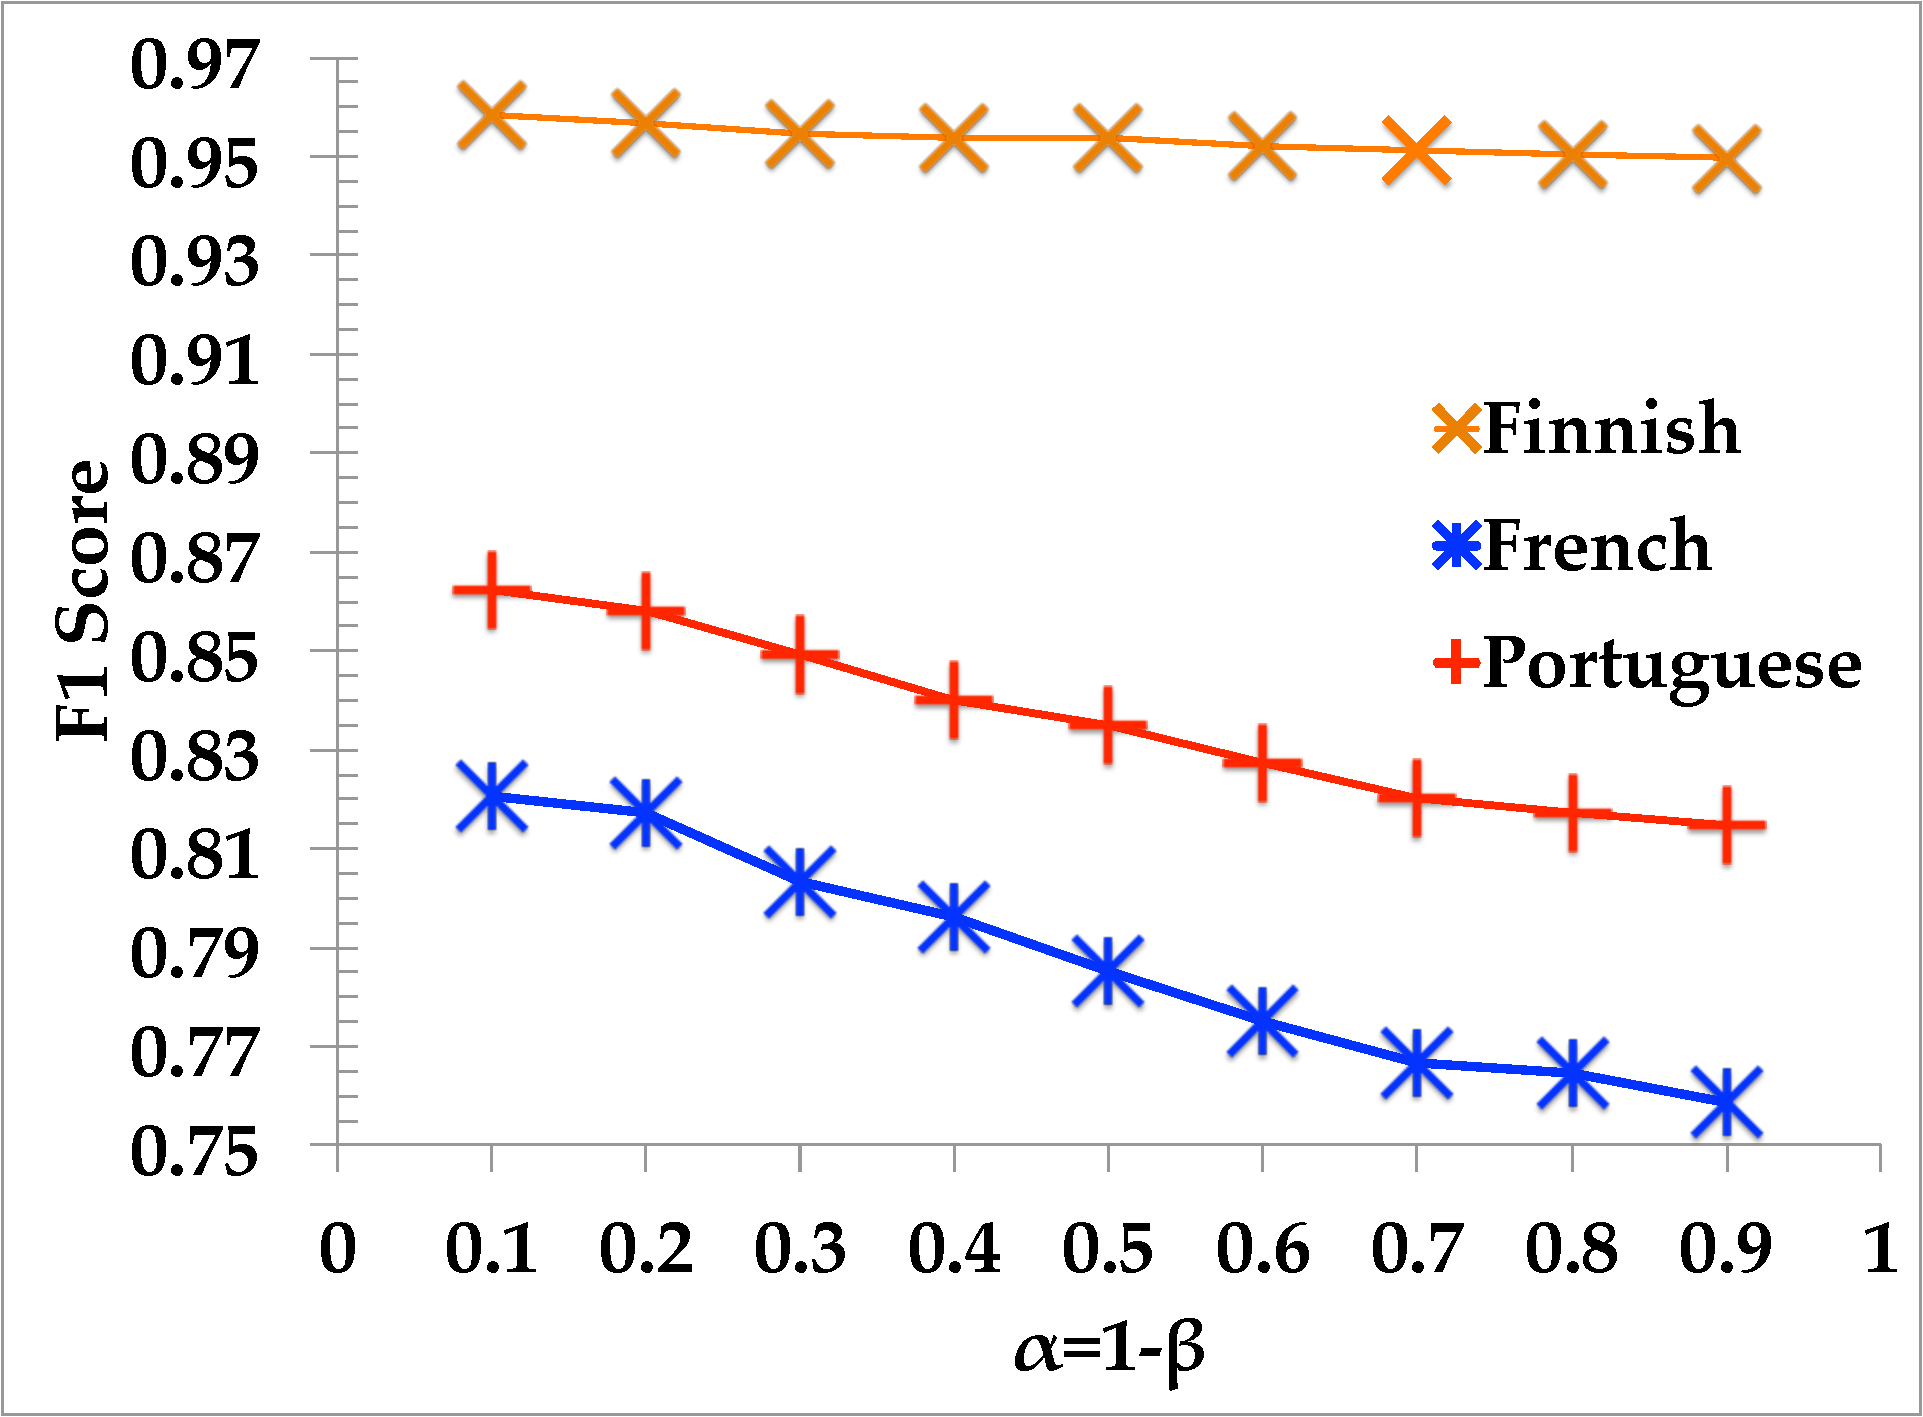
\includegraphics[width=0.30\columnwidth]{alphabetafig}
\caption{Score F1 pour le Finnois, le Français et le Portugais selon les valeurs de \(\alpha\) et \(\beta\).}
\label{fig.1}
\end{figure}

\subsubsection{Sélection du \(\delta\) optimal}
Maintenant que les valeurs optimales de  \(\alpha\) et \(\beta\) sont fixées, nous pouvons chercher pour la meilleure valeur de \(\delta\), que nous faisons varier par pas de \(0.05\) entre \(0\) et \(0.3\). Le choix de la borne supérieure est basé sur l'hypothèse que la valeur optimale est certainement plus proche de 0, car une seuil plus trop grand veut en fait dire que l'on sélectionnerait potentiellement tous les sens comme corrects, ce qui aurait pour effet de rajouter du bruit dans les résultats.

Comme  le \(\delta\) s'applique sur la fonction argmax nous pouvons aussi évaluer son effet sur d'autre mesures, parmi les mesures hybrides de niveau 2. Ici nous comparerons également l'indice de Tversky aux versions niveau deux des trois mesures de chaines approchées considérées lors de la première phase des expériences.
La figure 2 présente  les scores \(F_1\) pour chaque valeur de \(\delta\) et pour chaque langue d'évaluation. La première tendance que l'on observe, est que les mesures de niveau deux ont des performances clairement inférieures (jusqu'à 30\%) que notre mesure de Tversky. selon les langues, des valeurs différentes de \(delta\) sont optimales. Pour le français  \(\delta=0.10\), pour le finnois \(\delta=0.15\)
pour le portugais \(\delta=0.10\). 

Au travers de ces trois expériences, il est apparent que globalement, à part pour \(\delta\) (dont les variations sont tout de même dans une fenêtre assez petite), les valeurs optimales sont à peut près les mêmes, ce qui peut nous laisser penser qu'ils pourront bien se généraliser pour d autres langues. Cependant pour des langues comme le Chinois où le Japonais où la segmentation des mots n'est pas évidente, il semble raisonnable d'émettre l'hypothèse que les paramètres optimaux risquent d'être différents, en particulier sur le choix de la mesure de chaine approchée.

\subsection{Résultats de désambiguïsation finaux}

Maintenant que nous avons trouvé les paramètres et distances optimaux, nous pouvont extraire les résultats correspondants de l'expérience précédente et les placer dans la table \ref{tab:final} afin de faire une analyse plus poussée.Nous utilisons comme références pour la comparaison: la référence du sens le plus fréquent (MFS) et la référence aléatoire (Aléa).

La première chose remarquable est la différence conséquente entre le finnois et les deux autre langues, que ce soit au niveau des résultats de la désambiguïsation  où des références. En particulier, le fait que la référence aléatoire soit si haute suggère un faible niveau de polysémie, ce qui rend la tache de désambiguïsation bien plus aisée et explique bien les scores plus  élevés.

Une autre observation intéressante à faire est que, systématiquement la référence aléatoire à des scores supérieurs (jusqu'à \(6,6\%\)) à la référence du premier sens, ce qui laisse à penser que le premier sens est rarement le bon. Il se peut simplement que du fait de la nature collaborative de la ressource, on ne retrouve pas forcement un ordre des sens proportionnel à leur fréquence utilisation.

Si l'on s'intéresse aux résultats de l'état de l'art, nous atteignons une bonne performance par rapport aux travaux existants, avec une méthode relativement simple et peu couteuse à mettre en place.

\begin{table}
{\centering \footnotesize
\begin{tabular}{|c|c|c|c|c|c|}
\hline &P&R&F1&MFS F1&Aléa.\\
\hline Portuguese&0.8572&0.8814&0.8651&0.2397&0.3103\\
\hline Finnish&0.9642&0.9777&0.9687&0.7218&0.7962\\
\hline French&0.8267&0.8313&0.8263&0.3542&0.3767\\
\hline 
\end{tabular}
\caption{Résultat final avec la distance de chaine et les paramètre optimaux. Précision, Rappel, F-mesure for pour les trois langues comparés contre la référence du sens le plus fréquent et la référence aléatoire.}
\label{tab:final}
}
\end{table} 

\begin{figure}
\centering
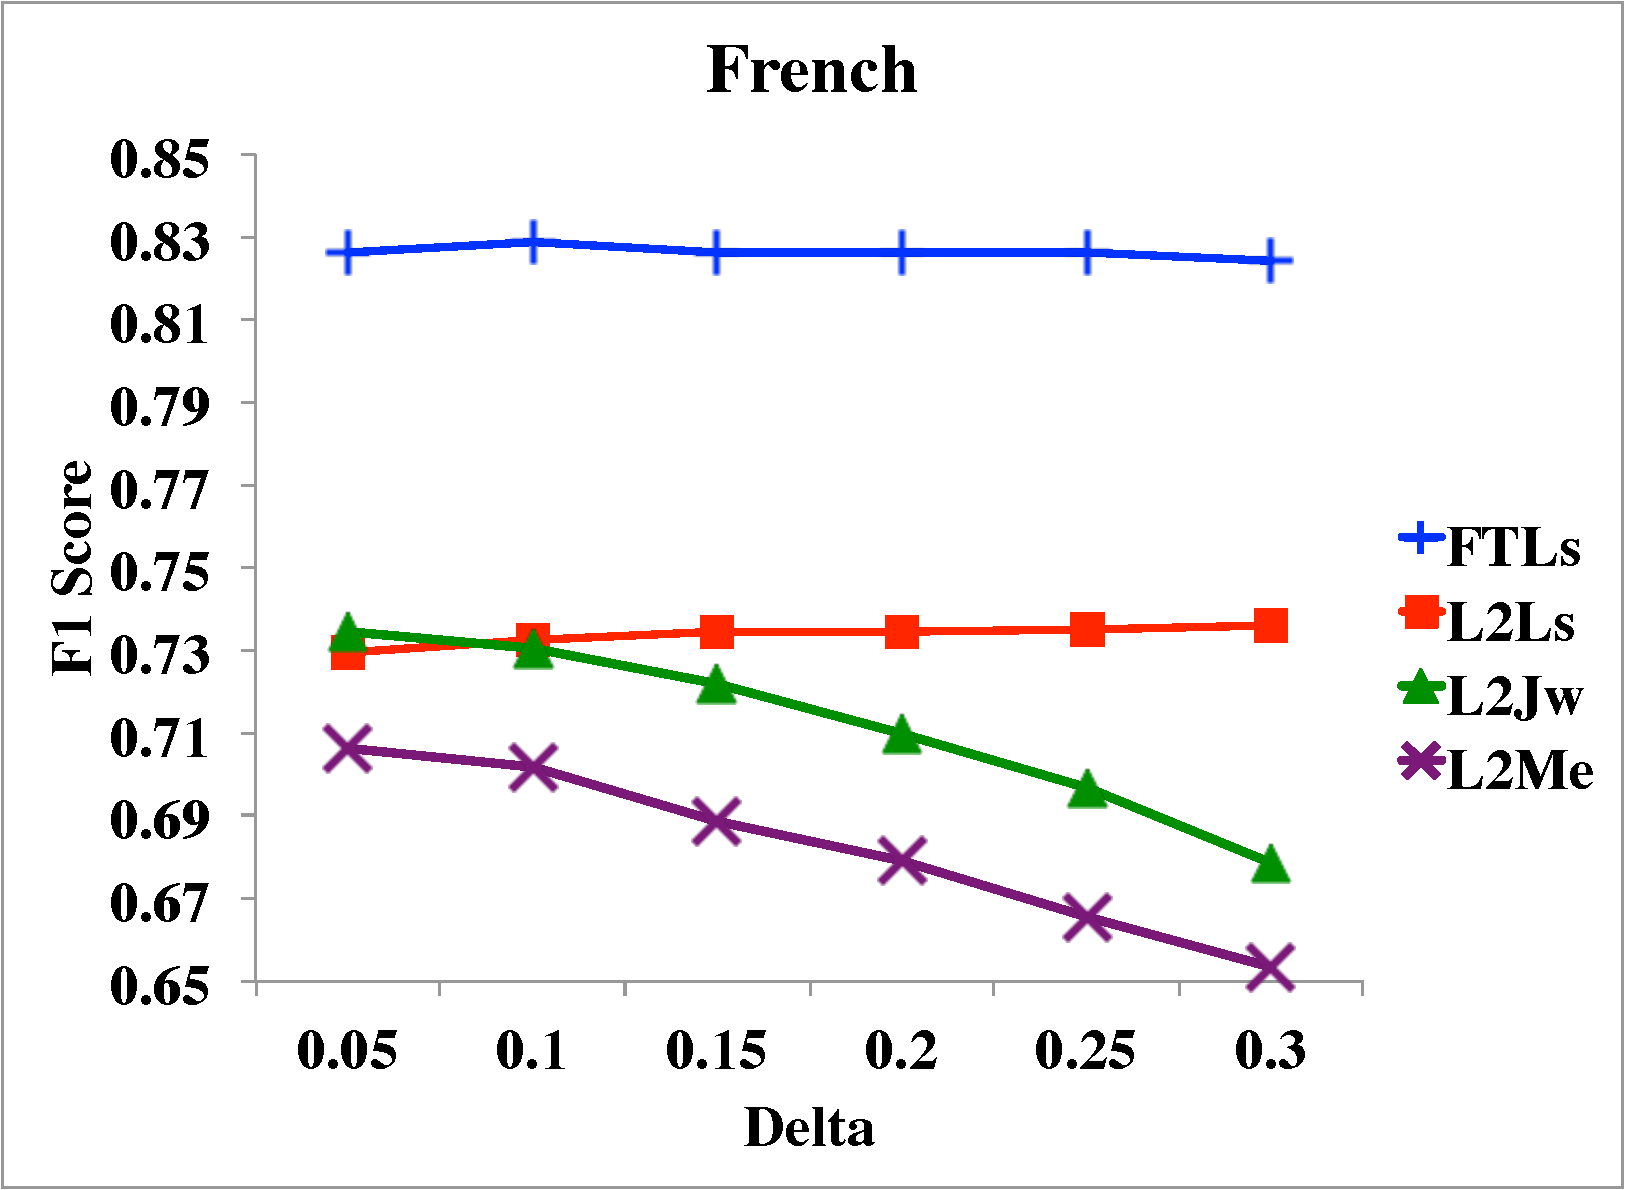
\includegraphics[width=.35\columnwidth]{french}
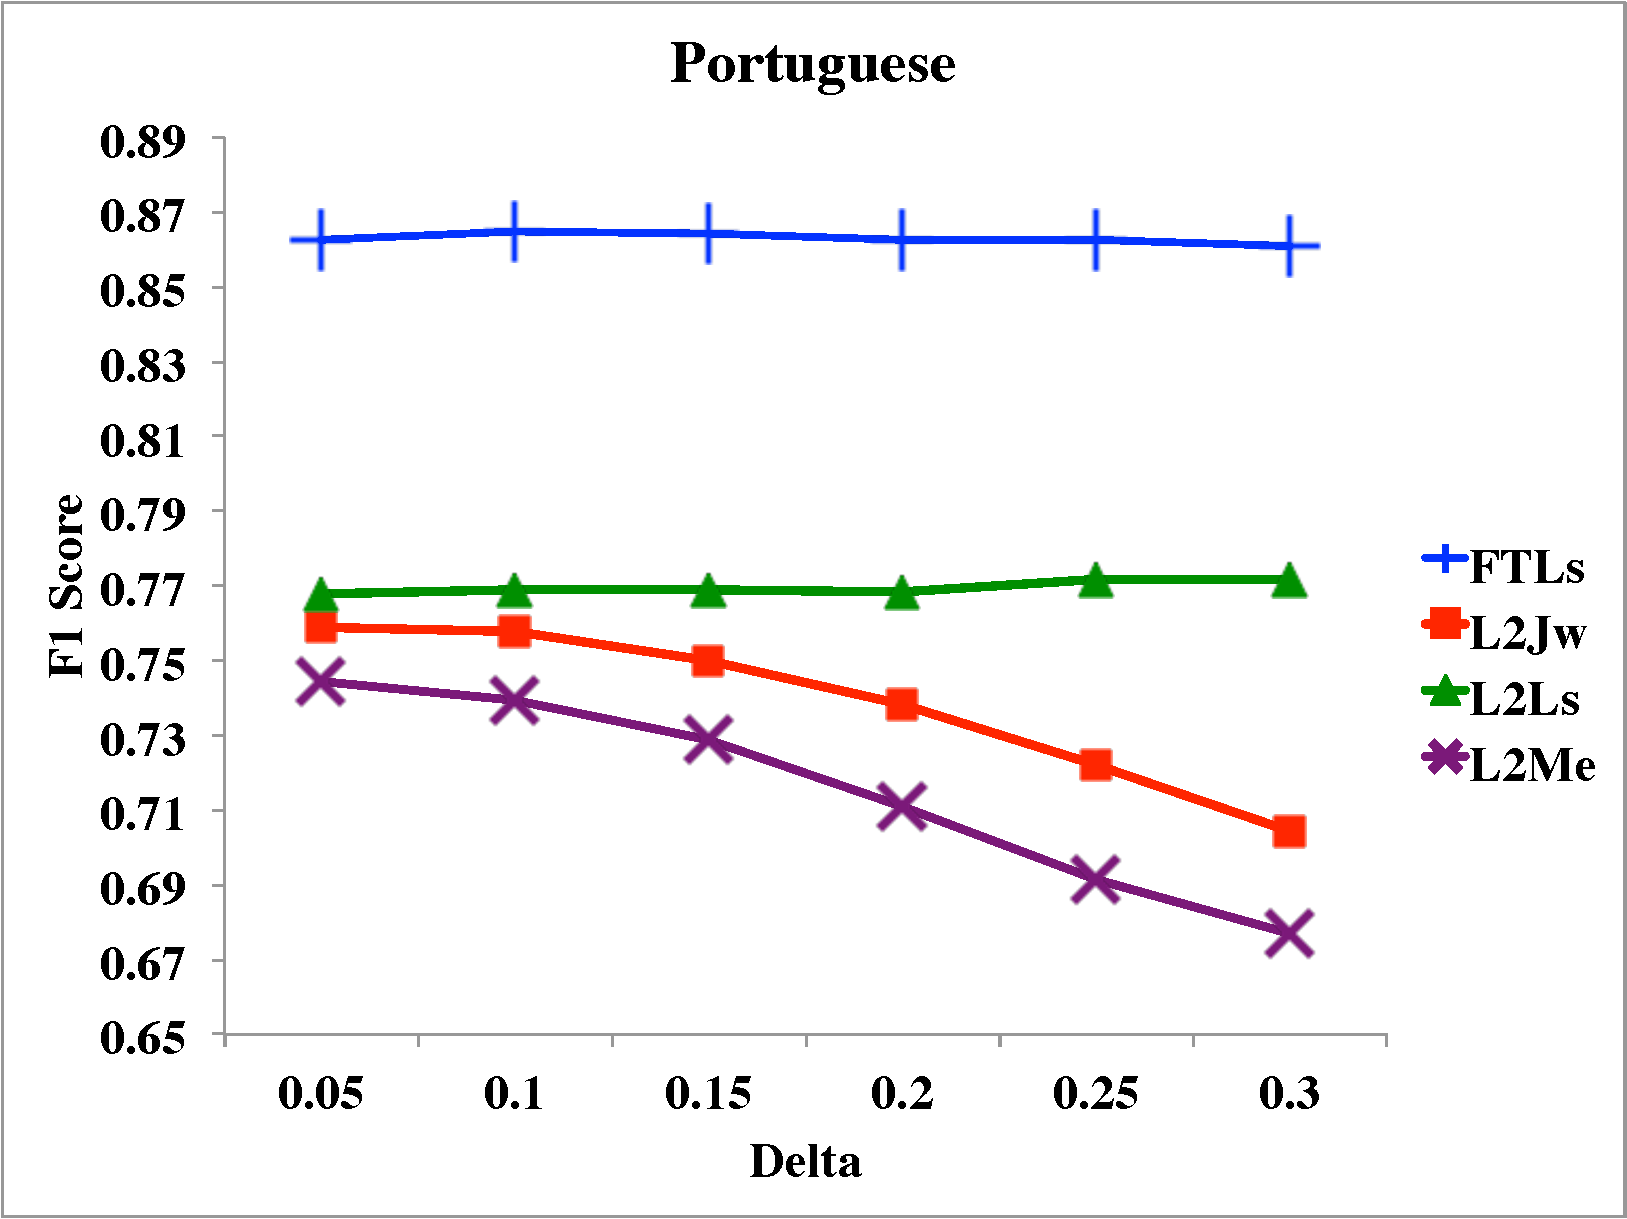
\includegraphics[width=.35\columnwidth]{portuguese}
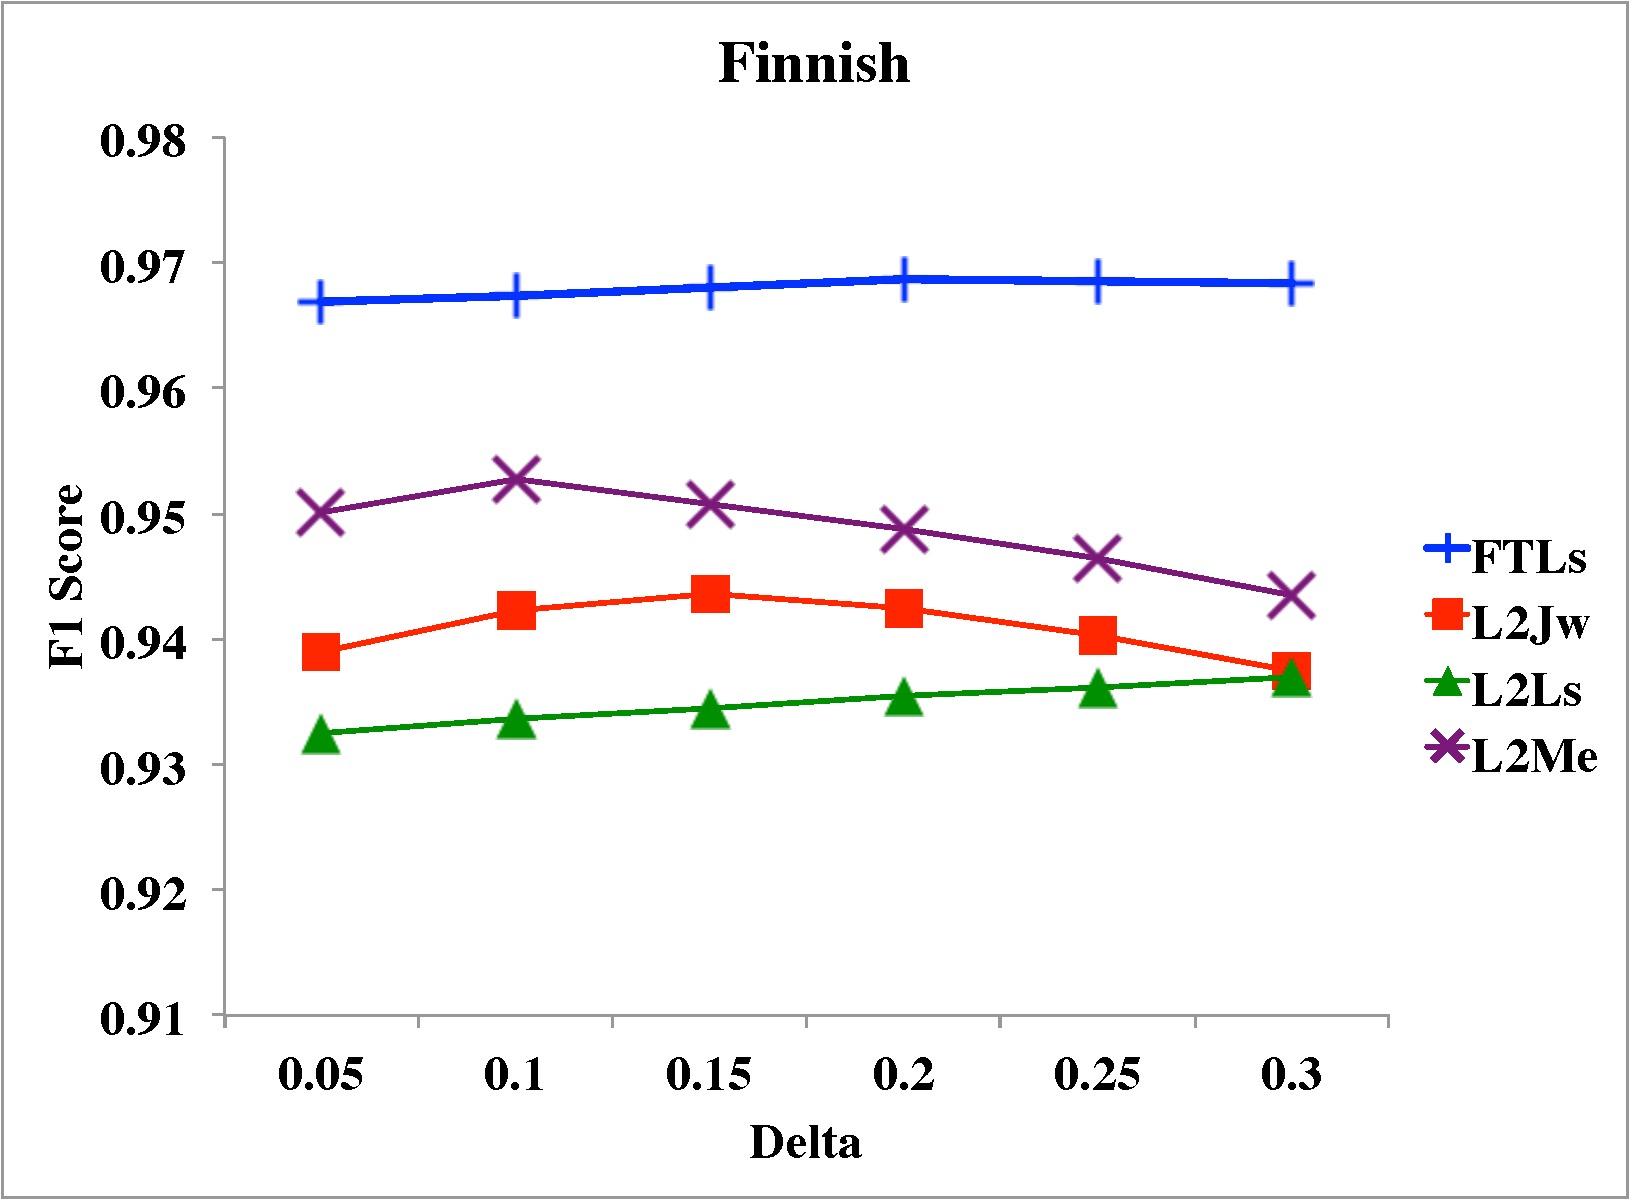
\includegraphics[width=.35\columnwidth]{finnish}
\caption{Représentation  graphique de la  F-mesure par rapports à la valeur de  delta pour notre mesure et les autres mesures de niveau 2.}
\label{fig.2}
\end{figure}

\subsection{Analyse d'erreurs}


Nous n'avons pas, ici effectué une analyse d'erreurs systématique, mais plutôt un échantillonnage manuel des erreurs, afin de se rendre compte des différents types d'erreur et de trouver des moyen de les détecter où même de les corriger.

Nous avons identifiés trois catégories d'erreurs principales:
\begin{enumerate}
\item Il n'y a pas de correspondance entre la glose et la définition du sens appropriée (résulte sur une choix aléatoire). Cette erreur survient lorsque la glose de la traduction est une paraphrase de la définition du sens où alors simplement métaphorique.
\item Il arrive que le seul mot en commun ne soit celui correspondant au domaine, qui est une information que nous n'extrayons pas à l'heure actuelle. Il en revient à catégoriser cette erreur comme cas particulier de la première.
\item Des nouveaux sens ont été introduits dans Wiktionary, ce qui a décalé tous les numéros de sens, qui n'ont pas été mis à jour ensuite. Ce type d'erreurs sont très difficiles à traiter.
\end{enumerate}

Nous pouvons en réalité par une méthode simple trouver les erreurs dues au manque de correspondance entre la glose et les définitions, et en modifiant le processus d'extraction actuel, nous pouvons éliminer les le deuxième type d'erreur.

Ainsi, il ne reste plus que les erreurs de la ressource originale qui sont dues à des inconsistances dans la mises à jour des pages. Nous pouvons alors aisément isoler et marquer ces erreurs pour que des humains aillent les corriger.

\section{Conclusion}

Avec la méthode que nous avons proposé, nous avons pu déterminer la mesure de similarité optimale pour la désambiguïsation des relation de traductions DBNary. Des résultats similaires dans les trois langues d'évaluation, suggèrent que cette estimation de paramètre optimaux se généralise bien et peuvent être appliqués au reste des langues présentes dans DBNary, sauf potentiellement dans des langues qui se segmentent difficilement, où d'autre paramètres seront certainement plus adaptés.

Enfin, en comparant les résultats nous pouvons conclure que notre méthode est adaptée pour la désambiguïsation de relations de traduction dans DBNary, surtout quand on considère que les références aléatoire et du sens le plus fréquent sont relativement basses, ce qui rend cette désambiguïsation un problème difficile.

Cependant, pour les relations sans glose, la procédure de désambiguïsation est plus complexe et fera partie des travaux futurs.


%%================================================================
%% Note : si l'on préfère éviter de factoriser les crossrefs :
%% bibtex -min-crossrefs 99 taln-exemple
%%================================================================
\bibliographystyle{taln2002}
\bibliography{taln-dbnary-wsd}

%%================================================================
\end{document}
